\section{Mise en oeuvre}%
\subsection{L'électronique}%
\subsubsection{Un jeu de LEGO}
Le montage est relativement simple; la carte RAMPS s'enffiche bien sur la Funduino. %
Il ne faut pas  assembler tout de suite les cartes. Il est préférable de fixer la %
funduino sur son support final (dans mon cas, une tole aluminum en équerre). une fois %
le Funduino fixée, on enffiche  la RAMPS (fig. \ref{montage_carte} %
page~\pageref{montage_carte}). il reste à brancher les commandes de moteur %
sur la RAMPS. Comme indiqué sur le wiki de Reprap, on vérifie les noms des broches et %
on branche (le GND va sur le GND et le direction va sur direction).%
\begin{figure}%
   \caption{\label{montage_carte} Montage de RAMPS sur la Funduino}%
   \center{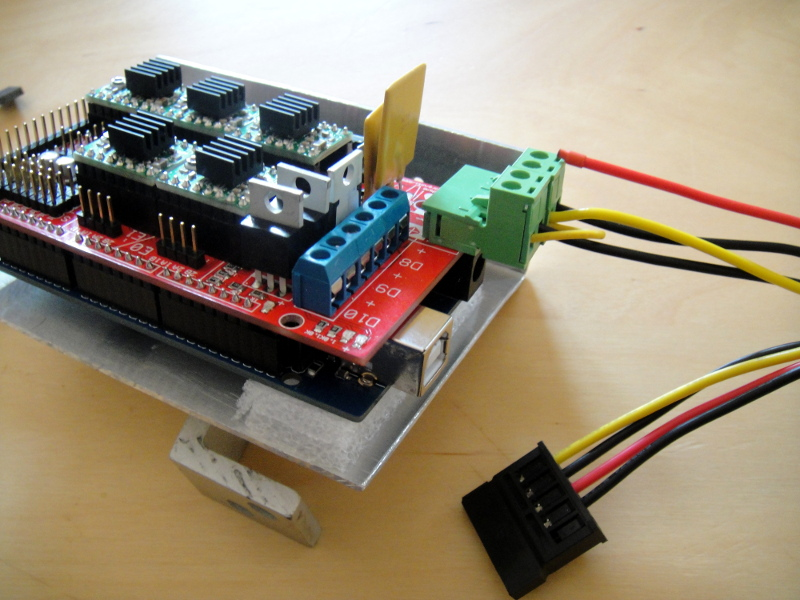
\includegraphics[width=10cm]{img/ramps02.jpg}}%
\end{figure}%
\subsubsection{Alimentation externe} %
Il faut maintenant l'alimentation externe sur la RAMPS (bornier vert à quatre broches). %
Il est préconisé d'alimenter en 12V. J'ai donc utilisé une alimentation de PC (500W, %
qui peut le plus, peu le moins). Pour info, le 0V, c'est le fil noir, le 12V, c'est le %
fil jaune. Comme d'habitude, l'alimentation de PC est un élément que j'ai trouvé %
dans un vide-grenier (5\euro{}). Il y a une entrée 5A et une entrée 11A. Mon %
alimentation a une capacité de 18A sur la sortie 12V. Il m'a donc suffit de mettre %
les deux entrées en parallèle sur le 12V fig. \ref{alimentation} %
page~\pageref{alimentation}).%
\begin{figure}%
   \caption{\label{alimentation} Branchement de l'alimentation externe}%
   \center{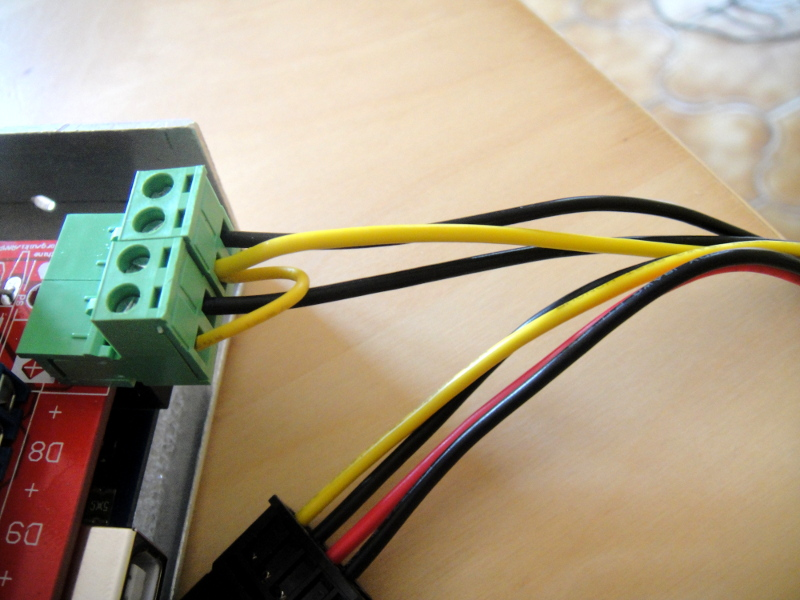
\includegraphics[width=10cm]{img/ramps03.jpg}}%
\end{figure}%
\subsubsection{Les premières embuches}
Ce qui devait arriver arriva. En faisant des essais sur la carte RAMPS, j'ai fait un %
court-circuit (5v relié au 0V). Une seconde a suffit pour que de la fumée s'échappe %
de la Funduino. Une %
fois l'ensemble démonté, un composant avait pris copieux. \par %
Diagnostique : quand je branche seul, le Funduino au PC avec le cordon USB, le %
périphérique est reconnu. Si maintenant, j'alimente la RAMPS en 12V, le PC perd la %
connection USB. C'est embêtant. Dans ces cas là, il faut garder son calme. La %
Funduino, tout comme l'Arduino est une carte super simple : il y a un micro controlleur, %
quelques résistances, un condensateur, parfois une interface USB (sinon, pris en charge %
par le micro controlleur), et ... un régulateur de tension (AMS1117). Ce régulateur de %
tension permet de garder 5V dans le circuit quelque soit la tension d'alimentation (tant %
qu'elle reste au dessus de 5V). C'est un composant à trois pattes équipé d'un radiateur, qui %
ressemble à une quatrième patte (fig. \ref{regulator} page~\pageref{regulator}). %
\begin{figure}%
   \caption{\label{regulator} Régulateurs de tension}%
   \center{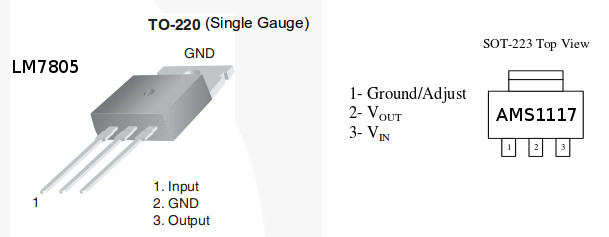
\includegraphics[width=10cm]{img/regulator.jpg}}%
\end{figure}%
En regardant bien, c'est ce composant qui a chargé. %
La réparation est simple : le LM7805 rempli la même fonction. Il est carrément plus gros, %
mais, on va trouver à le loger. J'en ai un sous le coude, c'est parti. Il faut être %
vigilent sur l'ordre des pattes. Pour s'adapter au circuit, il faut croiser le OUT %
et le GND pour avoir dans l'ordre [IN OUT GND] (fig. \ref{regulator} page~\pageref{regulator}). Ensuite on soude (fig. \ref{funduino_repared} %
page~\pageref{funduino_repared}). J'ai pris soin de mettre un scotch sur le radiateur du %
LM7805 pour éviter que la partie métallique ne touche une autre partie de la Funduino.\par{} %
Je rebranche le tout, et ... c'est reparti comme en 40 ! Ce qu'il faut retenir, c'est %
que la Funduino est très fragile (en même temps, un court-circuit ne pardonne pas), %
et qu'il faut vérifier à deux fois avant de brancher quelque chose (on ne branchera %
rien à chaud !).%
\begin{figure}%
   \caption{\label{funduino_repared} Funduino avec son nouveau régulateur de tension}%
   \center{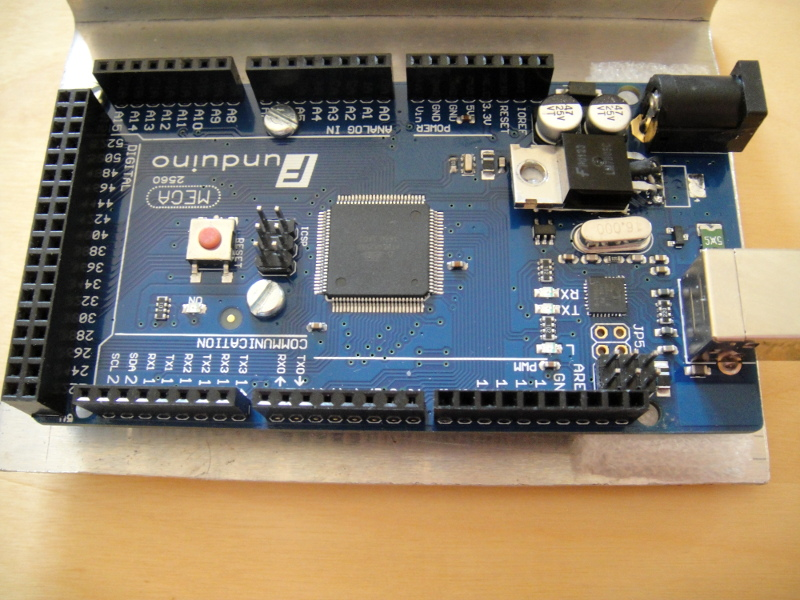
\includegraphics[width=10cm]{img/funduino02.jpg}}%
\end{figure}%